\documentclass[RNAAS]{aastex631}

% Numbers are \input from the pipeline-generated macros -- none typed by hand.
% Auto-generated by jansky_research.spectra._write_macros — do not edit by hand.
\newcommand{\usSource}{tgss-x-nvss @ <SkyCoord (ICRS): (ra, dec) in deg
    (180., 30.)>}
\newcommand{\usNmatched}{456}
\newcommand{\usAlphaMedian}{-0.73}
\newcommand{\usAlphaMin}{-1.65}
\newcommand{\usNuss}{6}
\newcommand{\usNinverted}{4}
\newcommand{\usThreshold}{-1.3}


\newcommand{\code}[1]{\texttt{#1}}

\begin{document}

\title{An Ultra-Steep-Spectrum Cut on TGSS~ADR1~$\times$~NVSS Is Neither Pure Nor
Complete}

\author[0009-0008-3289-4447]{Joseph Barbere}
\affiliation{Independent researcher}

\begin{abstract}
Ultra-steep-spectrum (USS) radio sources efficiently locate high-redshift radio
galaxies \citep{debreuck2000}. Using a small, tested tool (\code{spectra}), I
cross-match TGSS~ADR1 \citep{intema2017} with NVSS \citep{condon1998} in a
\usRadius$^\circ$ field, match \usNmatched\ sources (median $\alpha=\usAlphaMedian$),
and flag \usNuss\ raw USS candidates ($\alpha<\usThreshold$). Scored against the
\citet{degasperin2018} catalogue (built from the same uncorrected ADR1 fluxes), the
field shows no population offset ($+\usRealDeltaAlpha\pm\usRealDeltaAlphaSE$,
\usRealNPairs\ pairs), yet the candidates sit $\usRealFlaggedOffset$ steep, of which
a zero-free-parameter model of
selection on the noisy index predicts $\usRealSelPred\pm\usRealSelPredSD$. Against the reference's own USS population the cut is
\usRealPurityPct\% pure (\usRealNFlaggedRefUss\ of \usNuss) and \usRealCompletenessPct\%
complete (\usRealNRefUssRec\ of \usRealNRefUss), the disagreements being mostly sources at the
threshold and sources absent from our matched sample. A cautionary negative result.
\end{abstract}

\section{Result}

\code{spectra} \citep{jansky} is a pure-NumPy/Astropy tool that positionally
cross-matches TGSS and NVSS catalogue sources within $15\arcsec$, forms the two-point
index $\alpha_{150}^{1400}=\ln(S_{147.5}/S_{1400})/\ln(147.5/1400)$, and flags
$\alpha<\usThreshold$ as USS. Every routine is tested offline on a synthetic field
with injected indices, including sources injected at the cut. Run on a
\usRadius$^\circ$ cone at $(\usFieldRa^\circ,+\usFieldDec^\circ)$ near the North
Galactic Pole, it matches \usNmatched\ sources with a median $\alpha=\usAlphaMedian$,
consistent with flux-limited extragalactic samples, and flags \usNuss\ raw USS
candidates (steepest $\alpha=\usAlphaMin$), none with a measured redshift in NED or
SIMBAD (a manual check, not part of the committed pipeline).

The follow-up scores the whole field against the 1.4-million-source
\citet{degasperin2018} TGSS$\times$NVSS catalogue. That catalogue is built from the
same uncorrected ADR1 fluxes (its \S4 bounds the \citealt{hurleywalker2017}
flux-scale term at $\sim$0.06 in $\alpha$), so the comparison measures matching and
selection, not the flux scale. Three measured facts replace the flux-scale story an
earlier draft of this note told. The population shows no offset:
$+\usRealDeltaAlpha\pm\usRealDeltaAlphaSE$ over \usRealNPairs\ detection pairs,
consistent on both sides of the $+30^\circ$ declination edge of the rescaled-TGSS coverage. The
candidates still sit $\usRealFlaggedOffset$ below their reference values
(Figure~\ref{fig:spectra}; one candidate's reference entry is a non-detection limit,
excluded); treating the reference as truth and re-selecting on truth plus each
source's own noise predicts $\usRealSelPred\pm\usRealSelPredSD$, so the offset is consistent with
selection on the extreme of a noisy variable (a 1.3$\sigma$ residual; the model's central
value accounts for about half). The population null excludes a relative calibration
difference between the two catalogues, though not the ADR1 flux-scale term they share.
Against the reference's own single-component (\code{Scode=S}) USS population the cut is \usRealPurityPct\% pure
(\usRealNFlaggedRefUss\ of \usNuss) and \usRealCompletenessPct\% complete
(\usRealNRefUssRec\ of \usRealNRefUss). The committed rows show why. Of the five
candidates the reference does not confirm, one has only a non-detection limit there and two
have reference indices within 0.04 of the threshold; of the six missed
reference sources, three are absent from our matched sample, two lie within 0.012 of the
threshold, and one differs by 0.69 in $\alpha$ at a 7\arcsec\ separation. Since both
catalogues are built from the same two surveys, the survey floors cannot explain their
disagreement; they instead limit both against the true sky, where a joint detection is
equally sensitive only down to $\alpha\approx\usAlphaMatch$ and a source at
$\alpha=\usAlphaProbe$ must have $S_{150}\geq\usSNeededProbe$~mJy to be flagged at all.

A catalogue-level USS cut from this survey pair is therefore unreliable in both
directions. Every number above is \code{\textbackslash input} from a
pipeline-generated macro file, except the row-level counts and differences in the
preceding paragraph, which are tallied from the committed
\code{results/uss\_reference\_check.csv}; all regenerate from a clean checkout
(\code{python -m jansky\_research.spectra --ra \usFieldRa\ --dec \usFieldDec\
--radius \usRadius}).

\begin{figure}[h!]
\centering
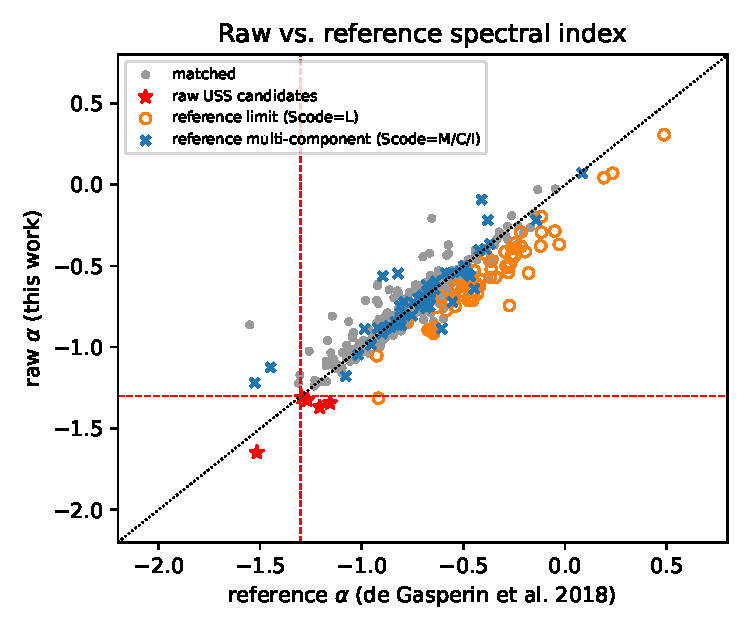
\includegraphics[width=0.7\linewidth]{figures/alpha_compare.pdf}
\caption{Raw spectral index against the \citet{degasperin2018} reference for every
matched source with a counterpart. The population lies on the identity line (mean
offset $+\usRealDeltaAlpha$); the raw USS candidates (stars) sit below it, part of
which the committed selection model predicts. Open circles are reference non-detection
limits (\code{Scode=L}, one of them a candidate) and crosses are multi-component entries
(\code{Scode=M/C/I}); only single-component detections enter the means and the
purity and completeness. Reference USS sources outside our matched sample cannot appear.}
\label{fig:spectra}
\end{figure}

\begin{acknowledgments}
Developed collaboratively with Anthropic's Claude \citep{anthropicclaude} (a large
language model); the author directed and verified the work, and an AI assistant is not
an eligible author. Thanks to the TGSS, NVSS, and de~Gasperin et al. teams for the
public catalogues.
\end{acknowledgments}

\software{jansky-research \citep{janskyresearch}, Astropy \citep{astropy2022}, NumPy,
SciPy, jansky \citep{jansky}}

\bibliographystyle{aasjournal}
\bibliography{refs}

\end{document}
